%%% File encoding: UTF-8
%%% äöüÄÖÜß  <-- keine deutschen Umlaute hier? UTF-faehigen Editor verwenden!

%%% Magic Comments zum Setzen der korrekten Parameter in kompatiblen IDEs
% !TeX encoding = utf8
% !TeX program = pdflatex 
% !TeX spellcheck = de_DE
% !BIB program = biber

\documentclass[bachelor,german,smartquotes]{hgbthesis}
% Zulässige Optionen in [..]: 
%   Typ der Arbeit: diploma, master (default), bachelor, internship
%   Hauptsprache: german (default), english
%	smartquotes: zur vereinfachten Eingabe von Hochkommas (nur "...")
%%%----------------------------------------------------------

\RequirePackage[utf8]{inputenc}		% bei der Verw. von lualatex oder xelatex entfernen!

\graphicspath{{images/}}    % Verzeichnis mit Bildern und Grafiken
\logofile{logo}				% Logo-Datei = images/logo.pdf (\logofile{}, wenn kein Logo gewünscht)
\bibliography{references}  	% Biblatex-Literaturdatei (references.bib)

%%%----------------------------------------------------------
% Angaben für die Titelei (Titelseite, Erklärung etc.)
%%%----------------------------------------------------------

% /* cSpell:enable */
% /* cSpell:locale de,en */

\title{Wirksamkeit der COVID-19-Impfung und Maßnahmen}
\author{Andreas Eckmayr}

\programtype{Fachhochschul-Bachelorstudiengang}

\programname{Medizin- und Bioinformatik}
\placeofstudy{Hagenberg}
\dateofsubmission{2022}{08}{31}

\advisor{FH-Prof. MMag. Dr. Gerald Lirk}

% /* cSpell:disable */

%\strictlicense		%%% restrictive license instead of Creative Commons (discouraged!)

%%%----------------------------------------------------------
\begin{document}
%%%----------------------------------------------------------

%%%----------------------------------------------------------
\frontmatter                    % Titelei (röm. Seitenzahlen)
%%%----------------------------------------------------------

\maketitle
\tableofcontents

%\chapter{Vorwort}

\begin{centering}

An dieser Stelle möchte ich mich bedanken bei\\
Magdalena\\
Eva, Robert, Christian und Barbara\\
Danke für Eure Unterstützung und Geduld!\\
Bei meinem Betreuer möchte ich mich
sehr herzlich für die motivierenden Worte bedanken.

\end{centering} 				% Vorwort ist optional
% /* cSpell:enable */
% /* cSpell:locale de,en */
\chapter{Kurzfassung}

In den letzten zweieinhalb Jahren haben wir uns alle zwangsweise mit Statistiken und dem Begriff Wirksamkeit auseinandersetzen müssen. Es existieren viele unterschiedliche Auffassungen darüber, was Wirksamkeit bedeutet. Diese Arbeit hat sich zum Ziel gesetzt, den Begriff der Wirksamkeit zu erläutern und zu veranschaulichen, aber auch die Frage, welche Maßnahmen und Impfstrategieen wirksam und erfolgreich waren, anhand zur Verfügung stehender Daten zu klären.

Im praktischen Teil der Arbeit wurden Zahlen aus verschiedenen Datensätzen verglichen und untersucht, ob sich daraus eine Wirksamkeit des Impfstoffes bzw. eine Wirksamkeit der Maßnahmenregelungen empirisch belegen lässt. Es wurden Korrelationen sowohl zwischen den verordneten Maßnahmen als auch zwischen der Impfquote und den Erkrankungs- bzw. Todesfällen gefunden.

Im Zuge der Arbeit wurde eine Onlinebefragung unter 425 TeilnehmerInnen durchgeführt, die dazu diente, die aktuellen Ansichten und Beweggründen der Bevölkerung abzubilden und mit den Zahlen und Fakten zu vergleichen. Es zeigte sich, dass die Beantwortung der Frage der Wirksamkeit vom Impfstatus und der Einstellung Impfungen gegenüber, nicht aber von der Bildung abhängig ist.
% /* cSpell:disable */		
% /* cSpell:enable */
% /* cSpell:locale en */
\chapter{Abstract}

\begin{english}

During the last two and a half years, we all had to deal with statistics, virology and the term effectiveness. A lot of different opinions and conceptions are existing around this term, yet not many people could explain it. The goal of this work is to explain and illustrate the term effectiveness but also to find an answer for the often asked question, which actions and vaccination strategies worked out.

For this, data from different sources was used and compared, and it was investigated if there is a correlation in this data. It was found that both vaccinations and stringency strongly correlated to cases and death numbers.

In the course of this work, an online survey of 425 people was conducted to find out which motives and opinions are actually out there. The results showed that people think differently whether the vaccination is effective or not depending on their own vaccination status and their take on vaccinations, education showed no impact.

\end{english}
% /* cSpell:disable */			

%%%----------------------------------------------------------
\mainmatter          % Hauptteil (ab hier arab. Seitenzahlen)
%%%----------------------------------------------------------

% /* cSpell:enable */
% /* cSpell:locale de,en */
\chapter{Einleitung}
\label{cha:Einleitung}

Seit Anfang 2020 beschäftigt uns nun COVID-19. Die Pandemie hat nicht nur zahlreiche Forschungsgebiete bewegt, sondern auch viele gesellschaftliche Fragen aufgeworfen. Von Beginn an standen Fragen wie "Welche Maßnahmen sind wirkungsvoll?" und "Auf welche Einschränkungen kann man verzichten?" im Diskussionsmittelpunkt. Dies betraf nicht nur die Forschung, sondern war immer auch ein Thema mit gesellschaftlicher Verantwortung. Sind Ausgehbeschränkungen notwendig, oder reicht es aus, Abstand zu halten? Ist die Ansteckungsgefahr in Schulen höher als in Büros? Welche Reisen sind weiterhin notwendig und unter welchen Voraussetzungen sollen diese möglich sein? Auf welche Dienstleistungen und Freizeitangebote können wir verzichten?
Diese Frage wird natürlich sehr individuell unterschiedlich beantwortet, deshalb ist es wichtig, einen gemeinschaftlichen Konsens zu finden.

Mit dem Aufkommen der Impfung hat sich dann auch die Frage gestellt, welcher Wirkstoff wirksamer ist oder ob überhaupt Impfstoffe wirksam sind. Dies war eng mit der Frage verknüpft, was Wirksamkeit denn eigentlich bedeutet. Bedeutet Wirksamkeit, dass die Ansteckungsgefahr gesenkt wird? Um wie viel muss die Ansteckungsgefahr gesenkt werden? Oder muss ein Impfstoff, um wirksam zu sein, lediglich Krankheitssymptome abmildern? Oder geht es um den Schutz von besonders vulnerablen Menschen? Welche Risiken dürfen hierbei in Kauf genommen werden?

\section{Der Begriff Wirksamkeit}
\label{sec:wirksamkeit}

Das Robert-Koch-Institut unterscheidet zwischen Impfstoffwirksamkeit und Impfstoffeffektivität und definiert diese beiden Begriffe wie folgt: \cite{rki-handbuch}

\begin{description}
    \item[Impfstoffeffektivität] "Die Gesamtauswirkungen des Einsatzes eines Impfstoffs; neben der direkten Impfstoffwirksamkeit können die indirekten Wirkungen der Impfung (wie die Reduktion der Inzidenz, Krankenhausbehandlungen, tödliche Ausgänge der Zielkrankheit) nach breiter Anwendung des Impfstoffs in einer Population unter Alltagsbedingungen in Studien ermittelt werden."

    \item[Impfstoffwirksamkeit] "Als direkte Wirkung des Impfstoffs wird die relative Reduktion des Risikos, nach Impfung im Vergleich zu Nichtgeimpften an der Zielkrankheit zu erkranken, vorzugsweise in kontrollierten Studien unter optimalen Bedingungen ermittelt. Als Maß für die Wirksamkeit eines Impfstoffs (IW) kann das Verhältnis der Erkrankungsquote bei Geimpften (EG) zu der bei Nichtgeimpften (ENG) ermittelt werden:"
    
    $IW(\%) = \frac{ENG-E}{ENG} \times 100$
\end{description}

Trotz dieser Definition sind Diskussionen über die Wirksamkeit neu entbrannt, aber auch über Impfpflichten und persönliche Rechte wurde debattiert.

\section{Krankheit und Virus}
\label{sec:virusinfo}
Die Krankheit COVID-19 wird vom Coronavirus SARS-CoV-2 verursacht. Bis jetzt gibt es zahlreiche Mutationen, die beobachtet werden. Zwei Varianten -- Delta und Omikron -- wurden vom "Centers for Disease Control and Prevention" (CDC) als "besorgniserregend" eingestuft, wobei erstere seit April wieder auf "beobachtet" zurückgestuft wurde. \cite{cdc-classification}
Die Übertragung erfolgt laut Robert Koch-Institut (RKI) vor allem über Respiration, eine Kontaktübertragung ist aber vor allem in unmittelbarer Umgebung infektiöser Personen nicht ausgeschlossen. Die Inkubationszeit beträgt im Median vier bis sechs Tage, häufige Symptome sind unter anderem Husten, Fieber, Schnupfen und Störung des Geruchs- und/oder Geschmackssinnes. Eine hohe Infektiösität besteht bereits vor dem Auftreten von Symptomen. Zur Einschränkung der Übertragung werden eine schnelle Isolierung positiver Personen, Identifizierung von Kontaktpersonen sowie Einhaltung von Hygieneregeln, das Tragen von Masken und Lüften empfohlen. Geimpfte Personen können sich prinzipiell infizieren und auch zu Überträgern werden, jedoch mit deutlich verringerter Wahrscheinlichkeit. \cite{rki}
Unter diesen Voraussetzungen ist zu erwarten, dass sowohl die COVID-19-Impfung als auch Einschränkungen von Veranstaltungen oder Ansammlungen sowie Reisebeschränkungen aktiv helfen, sowie diese Maßnahmen durch eine frühe Erkennung der Krankheit durch Tests oder Früherkennungssysteme die Fallzahlen senken.


\section{Verlauf der Pandemie}
\label{sec:pandemieverlauf}

Nach dem Ausbruch im Dezember 2019 wurde von der Weltgesundheitsorganisation WHO am 11. März 2020 die bis dahin als Epidemie eingestufte Krankheit offiziell zur weltweiten Pandemie erklärt. Kurz darauf wurden in Europa Maßnahmen beschlossen, um die weitere Verbreitung einzudämmen. Die im ersten Lockdown noch strengen Maßnahmen wurden im Sommer wieder gelockert, jedoch im Herbst, wenn auch weniger restriktiv, wieder eingeführt.

Im Dezember 2020 kamen zudem erste Impfstoffe auf, die im folgendem Sommer 2021 breit verfügbar waren.

Betrachtet man die Todesfälle (s. Abbildung \ref{fig:deaths}), so ist zu erkennen, dass es drei große Pandemiewellen gab -- von März bis Mai 2020, von Oktober 2020 bis Mai 2021 und von September/Oktober 2021 bis Mai 2022. Dabei kam in der zweiten Welle die Delta-Variante des Sars-CoV-2-Viruses auf, ab Dezember 2021 von der Omikron-Variante, die seither die vorherrschende Variante in Europa ist, verdrängt wurde. Vergleicht man die Todesfälle mit den Fallzahlen, wird deutlich, dass die Sterblichkeit des Virus dadurch abnahm.

\begin{figure}[ht]
    \caption{COVID-19-Fälle pro Million Einwohner seit Pandemiebeginn in Europa \cite{owidcoronavirus}}
    \label{fig:cases}
    \centering
    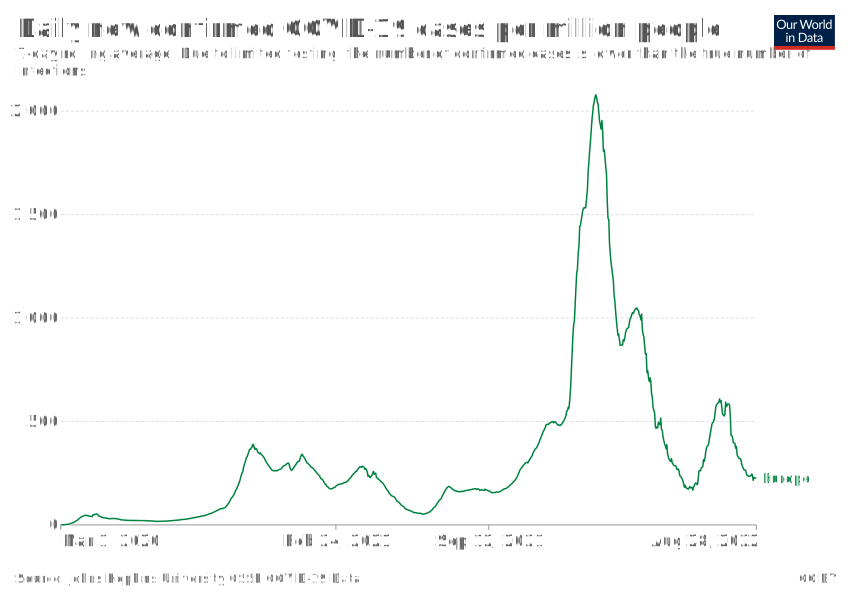
\includegraphics[trim={0 0 0 12cm},clip,width=0.6\linewidth]{coronavirus-data-explorer-europe}
\end{figure}

\begin{figure}[ht]
    \caption{Todesfälle pro Million Einwohner seit Pandemiebeginn in Europa \cite{owidcoronavirus}}
    \label{fig:deaths}
    \centering
    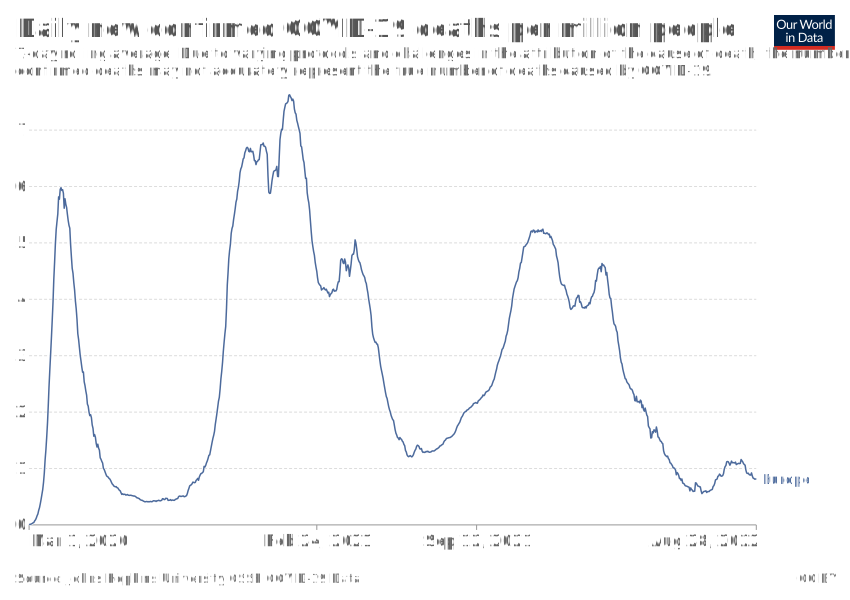
\includegraphics[trim={2cm 0 2cm 12cm},clip,width=0.6\linewidth]{coronavirus-data-explorer-deaths-europe}
\end{figure}

In der folgenden Arbeit werden die Zusammenhänge zwischen Fallzahlen, Maßnahmen und Impfrate untersucht, sowie eine Befragung zum Begriff Wirksamkeit durchgeführt. Die Frage, welche Maßnahmen wirkungsvoll waren und ob sich der Beitrag der Impfrate belegen lässt, sollen beantwortet werden.
% /* cSpell:disable */
% /* cSpell:enable */
% /* cSpell:locale de,en */
\chapter{Maßnahmen und Strategieen}
\label{cha:daten}

\section{Methodik}
\label{sec:datasets}

Als priorisierter Datensatz wurde das Angebot "Our World in Data" des Global Change Data Labs aus Großbritannien herangezogen. Die Organisation sammelt seit Pandemiebeginn Daten aus über 200 Ländern und bietet diese täglich aktualisiert zur freien Verwendung an. Pandemiedaten wie Fallzahlen, Todesfälle, Spitalsbelegungen und Testzahlen werden aus verschiedenen Quellen, unter anderem der nationalen Regierungen, dem European Centre for Disease Prevention and Control (ECDC), der Johns Hopkins University, gesammelt. Ergänzt werden diese unter anderem durch Daten wie Bruttoinlandsprodukt, durchschnittliche Lebenserwartung und Gesundheitsdaten von der Organisation for Economic Cooperation and Development (OECD) und der Weltbank, um eine demographische Beschreibung der Bevölkerung zur Verfügung zu stellen. \cite{owidcoronavirus}

Aus diesem Datensatz ist der "Stringency Index", ein errechneter Wert zwischen Null und 100, der Maßnahmen wie Schulschließungen, Versammlungsbeschränkungen, Reisebeschränkungen, Ausgangsbeschränkungen und Verordnungen an Arbeitsplätzen vergleicht und bewertet. Dabei sei betont, dass es sich bei diesem Wert um keine Beschreibung der Wirksamkeit der Maßnahmen handelt, sondern dieser nur zum Vergleich verschiedener Regionen und Staaten dient. \cite{oxcgrt}

Für Deutschland wurden zudem Daten des Projektes "Die Corona-Datenplattform" -- ein vom deutschem Bundesministerium für Wirtschaft und Klimaschutz in Auftrag gegebenes Projekt -- genutzt. Dieser Datensatz bietet im Vergleich zu "Our World in Data" eine genauere Auflösung, welche Maßnahmen genau gegolten haben und ist auch feingranularer bezüglich der exakt verimpften Impfstoffe. \cite{coronadatenplattform_de}

Für Österreich wurden die Daten aus dem COVID-19 Open Data Informationsportal genutzt. \cite{opendata_at}

Im Rahmen dieser Arbeit wurde die Datensatz-Beschreibung für den Datensatz von "Our World in Data" neu aufbereitet und für die verschiedenen Quellen ein Python-Skript mit Jupyter Code Cells als Schnittstelle zur Datenabfrage und Ausgabe erstellt. Dieses ist frei auf GitHub verfügbar.

\section{Ergebnisse}

Im folgenden wurde versucht, eine Korrelation zwischen Fallzahlen, Todesfällen, Maßnahmen (Stringency Index) und Impfzahlen zu finden. Verwendet wurden dazu die Korrelationskoeffizienten von Bravais-Pearson.

\subsection{Korrelation zwischen Fallzahlen und Todesfällen}

Betrachtet man die Todesfälle und die Fallzahlen, so fällt auf, dass diese Daten in Österreich und Deutschland miteinander korrelieren, in Großbritannien und Schweden ist dieser Effekt auch zu beobachten, jedoch schwächer ausgeprägt. Generell nahm diese Korrelation zwischen Fallzahlen und Todesfällen im Verlauf der Pandemie in Europa deutlich ab (siehe Tabellen in Anhang \ref{app:tabellen}). Im folgenden wurden speziell die Länder Österreich, Deutschland, Großbritannien und Schweden genauer untersucht.

\subsection{Maßnahmen zur Eindämmung der Pandemie}
\label{sec:massnahmen}

Der Stringency Index (s. Abbildung \ref{fig:stringency_index_comparison}) zeigt die in Kapitel \ref{sec:pandemieverlauf} erwähnten erlassenen und ausgesetzten Maßnahmen. Hier ist deutlich zu sehen, dass den Ruf, den Schweden hatte -- auf recht lockere Maßnahmen zu setzen -- nur bedingt wahr ist. Es wurden zwar lockerere Maßnahmen erlassen, diese dafür länger beibehalten. 
In Österreich und Deutschland wurden strengere Maßnahmen erlassen, welche aber schneller aufgehoben wurden.

\begin{figure}[ht]
    \caption{Stringency Index}
    \label{fig:stringency_index_comparison}
    \centering
    \includegraphics[trim={4cm 2cm 4cm 3cm},clip,width=\linewidth]{stringency_index_comparison2}
\end{figure}

Der Stringency Index korrelierte in jedem der untersuchten Staaten sowohl mit den Fallzahlen als auch mit den Todesfällen, wobei diese Korrelation nicht so stark wie erwartet und im Fall Großbritanniens sogar schwach ausgeprägt war.

Doch wie genau wurden Maßnahmen eingehalten? Dies lässt sich auch im Google Mobility Report beobachten - Besuche im Einzelhandel und Nutzung von Freizeitangeboten brach im ersten Lockdown um über 80\% ein, auch im öffentlichem Verkehr war ein Fahrgastzahlrückgang zu sehen - mit leichten Spitzen über die Weihnachtsfeiertage.
Interessant ist, dass allerdings in jedem Lockdown Familien- und Freundschaftsbesuche leicht zunahmen.
Im Arbeitsalltag lässt sich anhand der Daten beobachten, dass Home Office seit Pandemiebeginn zur Arbeitswelt dazugehört, hier sind Veränderungen zu sehen, die mit den aktuellen Fallzahlen einhergehen, eine Aktivität in den Büros wie vor der Pandemie wurde allerdings nicht mehr erreicht. \cite{google-mobility-report}

\begin{figure}[ht]
    \caption{Der Google Mobility Report zeigt die Umsetzung der Maßnahmen in Österreich}
    \label{fig:mobility_index_at}
    \centering
    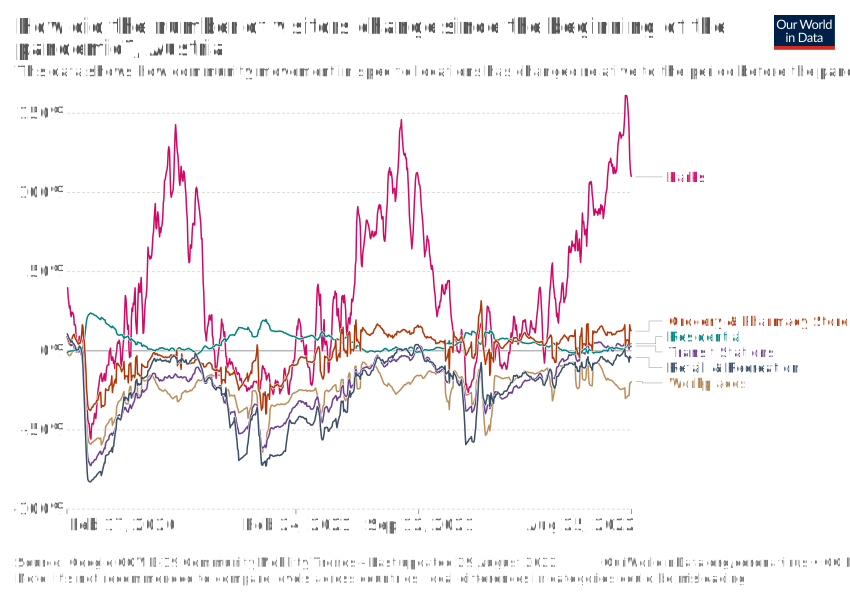
\includegraphics[trim={0 0 0 12cm},clip,width=\linewidth]{changes-visitors-covid-at}
\end{figure}

\subsection{Impfung gegen Sars-Cov-2}

Es konnte in jedem der untersuchten Länder eine starke Korrelation zwischen der Impfrate und den Fallzahlen bzw. den Todesfällen festgestellt werden. Diese war auch stärker als die Korrelation zwischen diesen Werten und dem Stringency Index.

\begin{figure}[ht]
    \caption{Neue Impfungen pro 100 Einwohner}
    \label{fig:vaccination_comparison}
    \centering
    \includegraphics[trim={4cm 2cm 4cm 2,5cm},clip,width=\linewidth]{vacc_comparison2}
\end{figure}


\begin{figure}[ht]
    \caption{Fallzahlen pro Million Einwohner}
    \label{fig:cases_comparison}
    \centering
    \includegraphics[trim={4cm 2cm 4cm 3cm},clip,width=\linewidth]{total_cases_comparison2}
\end{figure}


\begin{figure}[ht]
    \caption{Todesfälle pro Million Einwohner}
    \label{fig:death_comparison}
    \centering
    \includegraphics[trim={4cm 2cm 4cm 3cm},clip,width=\linewidth]{total_deaths_comparison2}
\end{figure}

\newpage

\section{Diskussion}

Es sind sowohl Korrelationen zwischen den Maßnahmen und den Fallzahlen als auch zwischen der Impfquote und den Fallzahlen zu beobachten. Interessant wäre eine Isolierung einzelner Maßnahmen. Dies gestaltete sich jedoch schwierig, da der Stringency Index bloß einen Anhaltspunkt bietet. Aus Deutschland liegen hierzu zwar sehr feingranulare Daten vorliegen, allerdings nie nur einzelne Maßnahmen, sondern immer ein Maßnahmenpaket erlassen wurde. In einer zukünftigen Arbeit könnten jedoch Daten aus einzelnen Bundesländern untersucht und verglichen werden. Eine alternative Herangehensweise könnte eine Untersuchung der Rohdaten des Stringency Index sein.

% /* cSpell:disable */
% /* cSpell:enable */
% /* cSpell:locale de,en */
\chapter{Umfrage}
\label{cha:umfrage}

Durch die Umfrage sollte die Bedeutung des Wortes Wirksamkeit in der Bevölkerung sowie die Einordnung der COVID-19-Impfung geklärt werden. Der Fragebogen besteht aus insgesamt 27 Fragen, davon sechs Fragen zur Erhebung über die Stichprobe. Die Ergebnisse wurden auf GitHub\footnote{\hyperlink{https://github.com/andreaseckmayr/BachelorThesis/blob/main/survey/Fragebogen\%20-\%20Wirksamkeit\%20d.\%20Covid-19\%20Impfung\%20(Responses)\%20-\%20Form\%20responses\%201.csv}{https://github.com/andreaseckmayr/BachelorThesis}} veröffentlicht.

\section{Methodik}

Die Umfrage wurde mit Google Forms erstellt. Die Stichprobengröße betrug 425 Personen und ergab sich durch Befragung des erweiterten Bekanntenkreises in den Gebieten Eferding und Purkersdorf. Die Umfrage wurde per Twitter, Facebook und WhatsApp verbreitet und online vom 14. April bis 1. Mai durchgeführt.
Das Alter der TeilnehmerInnen lag zwischen 14 und 83, dabei betrug der Mittelwert 47 Jahre und der Median 48 Jahre, der Modus 52 Jahre. 31\% der TeilnehmerInnen waren Männer, 69\% Frauen.
Im Vergleich dazu liegt das Durchschnittsalter der Bevölkerung in Österreich bei 43,1 Jahren, der Frauenanteil liegt bei 50,7\%.

\begin{figure}[hp]
    \centering
    \begin{tikzpicture}
        \pie[
            %color = {
            %    yellow!90!black,
            %    green!60!black,
            %    blue!60,
            %    red!70, 
            %    gray!70,
            %    teal!20},
            %hide number,
            text=legend,
            radius=2
        ]{
            31.1/männlich,
            68.7/weiblich,
            0.2/divers
        }
    \end{tikzpicture}
    \caption{Geschlechtsverteilung}
\end{figure}

\newpage

Betrachtet man die Stichprobe nach abgeschlossener Bildung, so stellt sie sich wie folgt dar:
\begin{itemize}
    \item 52\% haben eine Hochschule oder Universität abgeschlossenen
    \item 25\% haben eine Matura als höchste Ausbildung
    \item 11\% haben eine berufsbildende mittlere Schule (BMS) abgeschlossenen
    \item 10\% haben eine Lehre abgeschlossenen
    \item 2\% haben einen Pflichtschulabschluss
    \item weniger als 1\% hat noch keinen Abschluss
\end{itemize}

\begin{figure}[hp]
    \centering
    \begin{tikzpicture}
        \pie[
            %color = {
            %    yellow!90!black,
            %    green!60!black,
            %    blue!60,
            %    red!70, 
            %    gray!70,
            %    teal!20},
            %hide number,
            text=legend,
            radius=2.5
        ]{
            51.5/Hochschule; Universität,
            25.4/AHS; BHS; Abendmatura,
            10.6/BMS (Fach- od. Handelsschule),
            10.1/Lehre,
            1.9/Pflichtschule,
            0.5/noch kein Abschluss
        }
    \end{tikzpicture}
\caption{Höchste abgeschlossene Ausbildung}
\end{figure}

Gefragt wurde auch nach dem aktuellem Beruf. Dabei gaben zwei Drittel der Befragten an, unselbstständig angestellt zu sein. Davon sind 20\% leitende Angestellte und 4\% ArbeiterInnen. Jeweils ca. 15\% sind selbstständig oder derzeit nicht erwerbstätig und 5\% befinden sich noch in Ausbildung. Insgesamt 14\% der Befragten sind im Gesundheitsbereich tätig.

\begin{figure}[hp]
    \centering
    \begin{tikzpicture}
        \pie[
            %color = {
            %    yellow!90!black,
            %    green!60!black,
            %    blue!60,
            %    red!70, 
            %    gray!70,
            %    teal!20},
            %hide number,
            text=legend,
            radius=2.5
        ]{
            49.4/Angestellt,
            13.9/Leitendende Anstellung,
            2.8/ArbeiterIn,
            14.8/derzeit nicht erwerbstätig,
            14.6/Selbstständig,
            4.5/in Ausbildung
        }
    \end{tikzpicture}
\caption{Erwerbstätigkeit}
\end{figure}

\section{Ergebnisse}

\subsection{Impfwilligkeit und Wirksamkeit}

Um die Impfwilligkeit einzuschätzen, wurden die Teilnehmer befragt, unter welchen Umständen sie sich impfen lassen würden. Dabei stimmte der Aussage, sich gegen Krankheiten mit hohem Infektionsrisiko, aber leichten Krankheitssymptomen impfen zu lassen, ein Viertel gar nicht oder eher nicht zu, ein Fünftel war unentschlossen und 54\% stimmten eher bzw. völlig zu. Der konträren Aussage, sich gegen Krankheiten mit niedrigem Infektionsrisiko, allerdings schweren Krankheitssymptomen würde sich nur ein Zehntel nicht oder eher nicht impfen lassen, 13\% sind noch unentschlossen und 77\% antworteten mit ja oder eher ja.

Kurzzeitige Nebenwirkungen würden die meisten Menschen in Kauf nehmen, wobei fast 90\% leichte und 61\% auch noch schwere Nebenwirkungen akzeptieren würden. Länger andauernde Nebenwirkungen würde nur noch ein Viertel der Teilnehmer in Kauf nehmen.

Während 70\% der Befragten noch auf Empfehlungen der eigenen Ärztin oder des eigenen Arztes achten, gaben nur 61\% an, auch auf die Empfehlungen des Gesundheitsamtes oder der Impfkommission zu hören. 21\% waren gar der Meinung, auf die Empfehlung der Impfkommission eher nicht oder überhaupt nicht zu achten.

\begin{table}[h!]
    \centering
    \begin{tabular} {p{7.5cm} r r r r r}
        & 1 & 2 & 3 & 4 & 5 \\
        \hline
        Ich würde mich gegen Krankheiten mit\ldots & & & & & \\
        - hohem Infektionsrisiko, jedoch leichten Symptomen impfen lassen & 14,8\% & 12,0\% & 19,3\% & 20,7\% & 33,2\% \\

        - niedrigen Infektionsrisiko, jedoch schweren Symptomen impfen lassen & 5,6\% & 4,7\% & 12,9\% & 18,6\% & 58,1\% \\

        \\

        In Kauf nehme ich\ldots & & & & & \\

        - kurzzeitige leichte Nebenwirkungen wie Müdigkeit oder Schwindel & 2,8\% & 4,2\% & 5,4\% & 13,2\% & 74,4\% \\

        - kurzzeitige schwere Nebenwirkungen wie hohes Fieber & 10,4\% & 10,6\% & 18,1\% & 32,0\% & 28,9\% \\

        - länger andauernde Nebenwirkungen wie Müdigkeit & 20,5\% & 22,6\% & 28,7\% & 18,6\% & 9,6\% \\

        \\

        Vor einer Impfung achte ich auf\ldots & & & & & \\

        - Empfehlungen meiner Ärztin bzw. meines Arztes & 2,6\% & 8,0\% & 19,3\% & 28,7\% & 41,1\% \\

        - Empfehlungen des Gesundheitsamtes oder der Impfkommission & 9,9\% & 11,3\% & 17,9\% & 31,1\% & 29,9\% \\
    \end{tabular}
    \caption{Impfwilligkeit - Übersicht (1=ich stimme gar nicht zu, 5=ich stimme völlig zu)}
    \label{tab:impfwilligkeit}
\end{table}

Um wirksam zu sein, muss eine Impfung für fast 90\% der Befragten zumindest die Symptome mildern. Etwas weniger Zustimmung gab es zur Aussage, eine Impfung müsse das Infektionsrisiko senken (84\%) sowie die Wiedergabe des Erregers verhindern (80\%).

\begin{table}[h!]
    \centering
    \begin{tabular} {p{7.5cm} r r r r r}
        & 1 & 2 & 3 & 4 & 5 \\
        \hline
        Für mich ist eine Impfung wirksam\ldots & & & & & \\

        - wenn sie mein Infektionsrisiko senkt & 1,9\% & 4,2\% & 9,9\% & 26,6\% & 57,4\% \\

        - wenn sie die Weitergabe des Krankheitserregers verhindert & 2,1\% & 4,0\% & 13,9\% & 25,4\% & 54,6\% \\

        - wenn sie im Falle einer Infektion meine Symptome mildert & 2,1\% & 2,8\% & 8,0\% & 23,8\% & 63,3\% \\
    \end{tabular}
    \caption{Wirksamkeit - Übersicht (1=ich stimme gar nicht zu, 5=ich stimme völlig zu)}
    \label{tab:wirksamkeit}
\end{table}

\subsection{Gründe für eine Nicht-Impfung}

Zunächst wurden ungeimpfte Teilnehmer gefragt, was der Grund für eine Nicht-Impfung sei. Dabei standen folgende Antwortmöglichkeiten zur Auswahl:
\begin{itemize}
    \item religiöse Gründe
    \item gesundheitsbedingte Gründe
    \item generell vorsichtige Einstellung gegenüber Impfungen
    \item Angst vor Nebenwirkungen
\end{itemize}
Zwei Drittel der Befragten (62,9\%) gab an, Impfungen gegenüber generell vorsichtig eingestellt zu sein.
Rund ein Fünftel (22,9\%) gab an, Angst vor Nebenwirkungen zu haben.
14,3\% der TeilnehmerInnen gab gesundheitsbedingte Gründe an, die Religion war für keine Person Grund, sich nicht impfen zu wollen.
Diese Ergebnisse spiegeln sich teilweise in einer früheren forsa-Befragung wieder, in der knapp 18\% ebenfalls Angst vor Nebenwirkungen und 8\% gesundheitliche Gründe oder Schwangerschaft bzw. Stillzeit (5\%) angaben. Damals gaben allerdings lediglich 2\% Skepsis bzw. Ablehnung von Impfungen an, jedoch 34\% hielten Impfstoffe für nicht ausreichend erprobt. \cite{forsa-befragung}

\subsection{Gründe für eine Impfung}

Der Großteil der TeilnehmerInnen war zum Zeitpunkt der Umfrage bereits gegen COVID-19 geimpft. 81\% hatten die dritte Impfdosis -- den sogennanten Booster -- erhalten, 7\% wurden zwei mal geimpft. 9\% der Befragten waren noch ungeimpft.

Von den geimpften Personen haben sich vier Fünftel zum ehestmöglichen Zeitpunkt impfen lassen, 14\% haben einige Wochen verstreichen lassen und auf Reaktionen aus dem Freundes- und Bekanntenkreis gewartet. Zirka 3\% gab die Einführung von 3G am Arbeitsplatz, 1,6\% die Einführung von 2G in Gastronomie und Einzelhandel als Zeitpunkt an der Impfung an.

Nach den Gründen gefragt, war für beinahe 90\% der Selbstschutz ausschlaggebend, 76\% wollten besonders vulnerable Personengruppen schützen.  Leichter Reisen zu können war für ein Fünftel ein Impfgrund. 6\% gaben hier an, dass die 3G-Pflicht am Arbeitsplatz die Entscheidung beeinflusst hat, 5\% die 2G-Pflicht in Gastronomie und Einzelhandel.

\begin{table}[h!]
    \centering
    \begin{tabular} {p{12,5cm} r}
        Wann haben Sie sich impfen lassen? & \\
        \hline

        - Zum ehestmöglichen Zeitpunkt & 80,2\% \\

        - Nach ein paar Wochen, als bereits einige Freunde und Bekannte geimpft waren & 14,3\% \\

        - Mit der Einführung von 3G am Arbeitsplatz & 2,9\% \\

        - Mit der Einführung von 2G in der Gastronomie und im Handel & 1,6\% \\

        - Nach ein paar Wochen, aber aus dem Bekannten- und Familienkreis war ich der/die Erste & 1,0\% \\ \\

        Aus welchem Grund haben Sie sich impfen lassen? & \\
        \hline

        - Zu meinem eigenem Schutz & 88,8\% \\

        - Um besonders gefährdete Menschen zu schützen & 75,5\% \\

        - Um einfacher Reisen zu können & 17,5\% \\

        - Aufgrund der 3G-Pflicht am Arbeitsplatz & 5,5\% \\

        - Aufgrund der 2G/3G-Pflicht in Gastronomie und Handel & 5,2\% \\
    \end{tabular}
    \caption{Zeitpunkt der und Gründe für die COVID-19-Impfung - Übersicht}
    \label{tab:gruende}
\end{table}

\subsection{Vertrauen und Wirksamkeit bezüglich COVID-19-Impfung, Hygienemaßnahmen und Verordnungen}

Zuletzt wurden die TeilnehmerInnen gefragt, in welchen Bereichen Sie der COVID-19-Impfung vertrauen bzw. nicht vertrauen. Diese Bereiche waren wie folgt aufgeteilt:
\begin{itemize}
    \item Verhinderung einer Ansteckung
    \item Verminderte Symptome im Falle einer Ansteckung
    \item Geringere Wahrscheinlichkeit einer Weitergabe im Falle einer Ansteckung (Infektiösität)
    \item Keine der genannten
\end{itemize}

Es zeigt sich, dass die TeilnehmerInnen großteils darauf vertrauen, im Falle einer Ansteckung nicht bzw. mit schwächeren Symptomen zu erkranken (77\%). Nur die Hälfte glaubt, dass auch die Wahrscheinlichkeit einer Weiterverbreitung des Viruses gesenkt wird.

Gespalten waren die TeilnehmerInnen dabei, ob Hygienemaßnahmen bereits ausreichend wirksam seien - ein Viertel der Befragten meinte hierzu ja, 40\% hielten Hygienemaßnahmen für nicht ausreichend. Ähnlich war es bei den Verordnungen der Regierung fast die Hälfte (45\%) hielt diese für wirksam, ein Drittel meinte dazu, diese Maßnahmen seien nicht wirksam.

\begin{table}[h!]
    \centering
    \begin{tabular} {p{9.5cm} r r}
        In welchen Bereichen vertrauen Sie der COVID-19-Impfung? & Vertrauen & Kein Vertrauen \\
        \hline

        - Verhinderung einer Ansteckung & 28,9\% & 63,3\% \\

        - Verminderte Symptome im Falle einer Ansteckung & 76,7\% & 17,2\% \\

        - Geringere Wahrscheinlichkeit einer Weitergabe im Falle einer Ansteckung & 50,8\% & 36,0\% \\

        - Keine der genannten & 16,7\% & 29,2\% \\
    \end{tabular}
    \caption{Vertrauen in die COVID-19-Impfung - Übersicht (1=ich stimme gar nicht zu, 5=ich stimme völlig zu)}
    \label{tab:vertrauen}
\end{table}

\begin{table}[h!]
    \centering
    \begin{tabular} {p{7.5cm} r r r r r}
        & 1 & 2 & 3 & 4 & 5 \\
        \hline
         & & & & & \\

        - Sind generelle Hygienemaßnahmen (Sicherheitsabstände, Hände waschen, Lüften, persönliche Schutzmaßnahmen) Ihrer Ansicht nach bereits ausreichend wirksam?
        & 12,9\% & 26,4\% & 35,1\% & 18,6\% & 7,1\% \\

        - Sind COVID-19-Maßnahmen der Regierung (Einschränkungen für Gastronomie, Veranstaltungen, Home Office) Ihrer Ansicht nach wirksam?
        & 12,0\% & 17,6\% & 26,1\% & 28,9\% & 15,3\% \\
    \end{tabular}
    \caption{Wirksamkeit von Hygienemaßnahmen und Verordnungen - Übersicht (1=ich stimme gar nicht zu, 5=ich stimme völlig zu)}
    \label{tab:vertrauen2}
\end{table}

Im folgenden wurden die quantitativen Daten aus der Umfrage auf mögliche Zusammenhänge zwischen demographischen Daten und Meinungen untersucht. Dazu wurde der Chi-Quadrat-Test (\(\chi^2\)) eingesetzt.

\subsection{Zusammenhänge mit dem Impfstatus}

Die Werte wurden in "geimpft" und "ungeimpft" klassifiziert, wobei "geimpft" alle Personen beinhaltet, die zumindest eine COVID-19-Impfung erhalten haben.

Als Nullhypothese \(H_0\) wird angenommen, dass der Impfstatus keinen Einfluss auf die Einschätzung, ob die Impfung das Infektionsrisiko senkt (1), die Weitergabe verhindert (2) oder die Symptome mildert (3) nimmt.

Der kritische Wert beträgt \(df = 9,488\) für eine Signifikanz \(p = 0,05\).
Für die erste Nullhypothese wurde \(\chi^2 = 68,411\) mit einer Signifikanz \(p = 0\) ermittelt. Für die zweite Nullhypothese wurde \(\chi^2 = 16,764\) mit einer Signifikanz \(p = 0,002\) berechnet. Für die dritte Nullhypothese ergibt \(\chi^2 = 116,457\) mit einer Signifikanz von \(p = 0\). Somit müssen alle drei Nullhypothesen abgelehnt werden. Der Impfstatus beeinflusst also die Antwort auf die Frage, wann eine Impfung wirksam ist.

\begin{figure}[ht]
    \caption{Für mich ist eine Impfung wirksam, wenn sie mein Infektionsrisiko senkt. - Nach Alter gruppiert}
    \label{fig:vgl_infektionsrisiko_impfstatus}
    \centering
    \includegraphics[trim={0 0 0 0.9cm},clip,width=.7\linewidth]{data_infektionsrisiko_impfstatus}
\end{figure}

\begin{figure}[ht]
    \caption{Für mich ist eine Impfung wirksam, wenn sie die Weitergabe des Krankheitserregers verhindert. - Nach Alter gruppiert}
    \label{fig:vgl_weitergabe_impfstatus}
    \centering
    \includegraphics[trim={0 0 0 0.9cm},clip,width=.7\linewidth]{data_weitergabe_impfstatus}
\end{figure}

\begin{figure}[ht]
    \caption{Für mich ist eine Impfung wirksam, wenn sie im Falle einer Infektion meine Symptome mildert. - Nach Alter gruppiert}
    \label{fig:vgl_symptome_impfstatus}
    \centering
    \includegraphics[trim={0 0 0 0.9cm},clip,width=.7\linewidth]{data_symptome_impfstatus}
\end{figure}

Weiters wurde die Nullhypothese angenommen, dass der Impfstatus einer Person keine Rolle spielt, ob man bereits Hygienemaßnahmen oder für ausreichend hält und ob man Maßnahmenverordnungen für wirksam hält.

Für erstere Nullhypothese wurde \(\chi^2 = 56,645\) mit einer Signifikanz von \(p = 0\), für zweitere \(\chi^2 = 105,903\) und \(p = 0\) errechnet. Damit werden beide Nullhypothesen abgelehnt, der hat also einen Einfluss auf genannte Ansichten.

Zuletzt wurde angenommen, dass der Impfstatus keinen Einfluss darauf hat, in welchen Bereichen man die COVID-19-Impfung für wirksam bzw. nicht wirksam hält. Die erste Hypothese wurde mit \(\chi^2 = 196,679\) und \(p = 0\) abgelehnt, die zweite Hypothese wurde mit \(\chi^2 = 7,815\) und \(p = 0,023\) ebenfalls abgelehnt. Der kritische Wert lag für diese Hypothesen bei 7,815.

\subsection{Zusammenhänge mit der Bildung}

Die Werte wurden in folgende Klassen eingeteilt:
\begin{itemize}
    \item Hochschule
    \item Matura
    \item Berufsbildende Mittlere Schule und Lehre
    \item Sonst
\end{itemize}

Als Nullhypothese \(H_0\) wird angenommen, dass die Bildungsstufe keinen Einfluss auf die Einschätzung der Wirksamkeit nimmt.

Der kritische Wert beträgt \(df = 21,026\) für eine Signifikanz \(p = 0,05\).
Für die erste Nullhypothese wurde \(\chi^2 = 19,770\) mit einer Signifikanz \(p = 0,072\) ermittelt. Für die zweite Nullhypothese wurde \(\chi^2 = 14,859\) mit einer Signifikanz \(p = 0,249\) berechnet. Für die dritte Nullhypothese ergibt \(\chi^2 = 19,421\) mit einer Signifikanz von \(p = 0,079\). Keine der drei Nullhypothesen kann abgelehnt werden, daraus folgt, dass die Bildung tatsächlich keine Auswirkung darauf hat, wie jemand die Wirksamkeit der Impfung einschätzt.

\begin{figure}[ht]
    \caption{Für mich ist eine Impfung wirksam, wenn sie mein Infektionsrisiko senkt. - Nach Bildung gruppiert}
    \label{fig:vgl_infektionsrisiko_bildung}
    \centering
    \includegraphics[trim={0 0 0 0.9cm},clip,width=.9\linewidth]{data_infektionsrisiko_bildung}
\end{figure}

\begin{figure}[ht]
    \caption{Für mich ist eine Impfung wirksam, wenn sie die Weitergabe des Krankheitserregers verhindert. - Nach Bildung gruppiert}
    \label{fig:vgl_weitergabe_bildung}
    \centering
    \includegraphics[trim={0 0 0 0.9cm},clip,width=.9\linewidth]{data_weitergabe_bildung}
\end{figure}

\begin{figure}[ht]
    \caption{Für mich ist eine Impfung wirksam, wenn sie im Falle einer Infektion meine Symptome mildert. - Nach Bildung gruppiert}
    \label{fig:vgl_symptome_bildung}
    \centering
    \includegraphics[trim={0 0 0 0.9cm},clip,width=.9\linewidth]{data_symptome_bildung}
\end{figure}

\subsection{Zusammenhänge mit dem Alter}

Die Werte wurden in folgende Altersklassen eingeteilt:
\begin{itemize}
    \item 0 bis 29 Jahre
    \item 30 bis 44 Jahre
    \item 45 bis 64 Jahre
    \item 65 Jahre oder älter
\end{itemize}
Als Nullhypothese \(H_0\) wird angenommen, dass das Alter keine Auswirkung auf die Einschätzung der Wirksamkeit hat.
Der kritische Wert beträgt \(df = 21,026\) für eine Signifikanz \(p = 0,05\). Bei der ersten Aussage ergab \(\chi^2 = 27,849\) mit einer Signifikanz \(p = 0,006\). Damit muss diese Nullhypothese abgelehnt werden.
Bei der zweiten Aussage konnte \(\chi^2 = 9,781\) mit einer Signifikanz von \(p = 0,635\) berechnet werden. Diese Nullhypothese kann folglich nicht abgelehnt werden.
Bei der dritten Aussage wurde  \(\chi^2 = 22,714\) mit einer Signifikanz von \(p = 0,03\) ermittelt. Diese Nullhypothese muss ebenfalls abgelehnt werden.

Damit wird die Nullhypothese abgelehnt, folglich gibt es einen Zusammenhang zwischen der Aussage "Für mich ist eine Impfung wirksam, wenn sie mein Infektionsrisiko senkt." und dem Alter.

Die zweite Nullhypothese -- das Alter hat keine Auswirkung auf die Zustimmung der Aussage "Für mich ist eine Impfung wirksam, wenn sie die Weitergabe des Krankheitserregers verhindert." -- wird beibehalten.

Die dritte Nullhypothese -- das Alter hat keine Auswirkung auf die Zustimmung der Aussage "Für mich ist eine Impfung wirksam, wenn sie im Falle einer Infektion meine Symptome mildert." -- wird abgelehnt.

\begin{figure}[ht]
    \caption{Für mich ist eine Impfung wirksam, wenn sie mein Infektionsrisiko senkt. - Nach Alter gruppiert}
    \label{fig:vgl_infektionsrisiko_altersgruppen}
    \centering
    \includegraphics[trim={0 0 0 0.9cm},clip,width=.9\linewidth]{data_infektionsrisiko_altersgruppen}
\end{figure}

\begin{figure}[ht]
    \caption{Für mich ist eine Impfung wirksam, wenn sie die Weitergabe des Krankheitserregers verhindert. - Nach Alter gruppiert}
    \label{fig:vgl_weitergabe_altersgruppen}
    \centering
    \includegraphics[trim={0 0 0 0.9cm},clip,width=.9\linewidth]{data_weitergabe_altersgruppen}
\end{figure}

\begin{figure}[ht]
    \caption{Für mich ist eine Impfung wirksam, wenn sie im Falle einer Infektion meine Symptome mildert. - Nach Alter gruppiert}
    \label{fig:vgl_symptome_altersgruppen}
    \centering
    \includegraphics[trim={0 0 0 0.9cm},clip,width=.9\linewidth]{data_symptome_altersgruppen}
\end{figure}

\newpage

\section{Diskussion}

Es wurden Einflüsse des Alters und vor allem des Impfstatus auf die Einstellung bzw. Beurteilung der Maßnahmen und der Wirksamkeit der Impfung gezeigt. Die Bildung selber hatte dabei keinen entscheidenden Einfluss.
Interessant wäre dabei allerdings eine Beobachtung über längere Zeiträume und ob neue Erkenntnisse diese Meinung beeinflussen können.

\begin{table}[h!]
    \centering
    \begin{tabular} {p{9cm} | r | r | r}
        Nullhypothese & $\chi^2$ & p & Status \\
        \hline
        Der Impfstatus hat keinen Einfluss auf die Beurteilung der Wirksamkeit bzgl. Senkung des Infektionsrisikos. & 68,411 & 0,000 & abgelehnt \\
        Der Impfstatus hat keinen Einfluss auf die Beurteilung der Wirksamkeit bzgl. Weitergabe des Virus. & 16,764 & 0,002 & abgelehnt \\
        Der Impfstatus hat keinen Einfluss auf die Beurteilung der Wirksamkeit bzgl. Milderung der Symptome. & 116,457 & 0,000 & abgelehnt \\

        Der Impfstatus hat keinen Einfluss darauf, ob man einfache Hygienemaßnahmen als Maßnahme bereits für ausreichend hält. & 56,645 & 0,000 & abgelehnt \\
        Der Impfstatus hat keinen Einfluss darauf, ob man die Maßnahmenverordnung für wirksam hält. & 105,903 & 0,000 & abgelehnt \\

        Der Impfstatus hat keinen Einfluss darauf, in welchen Bereichen man die COVID-19-Impfung für wirksam hält. & 196,679 & 0,000 & abgelehnt \\
        Der Impfstatus hat keinen Einfluss darauf, in welchen Bereichen man die COVID-19-Impfung für nicht wirksam hält. & 9,552 & 0,023 & abgelehnt \\

        Die Bildung hat keinen Einfluss auf die Beurteilung der Wirksamkeit bzgl. Senkung des Infektionsrisikos. & 19,770 & 0,072 & angenommen \\
        Die Bildung hat keinen Einfluss auf die Beurteilung der Wirksamkeit bzgl. Weitergabe des Virus. & 14,859 & 0,249 & angenommen \\
        Die Bildung hat keinen Einfluss auf die Beurteilung der Wirksamkeit bzgl. Milderung der Symptome. & 19,421 & 0,000 & angenommen \\

        Das Alter hat keinen Einfluss auf die Beurteilung der Wirksamkeit bzgl. Senkung des Infektionsrisikos. & 27,849 & 0,006 & abgelehnt \\
        Das Alter hat keinen Einfluss auf die Beurteilung der Wirksamkeit bzgl. Weitergabe des Virus. & 9,781 & 0,635 & angenommen \\
        Das Alter hat keinen Einfluss auf die Beurteilung der Wirksamkeit bzgl. Milderung der Symptome. & 22,714 & 0,030 & abgelehnt \\

    \end{tabular}
    \caption{Aufgestellte Nullhypothesen - Übersicht}
    \label{tab:hypothesen}
\end{table}
% /* cSpell:disable */
% /* cSpell:enable */
% /* cSpell:locale de,en */
\chapter{Schlussbemerkungen}
\label{cha:Schluss}

Im Rahmen dieser Arbeit wurde ein Python-Skript mit Jupyter Code Cells zur Abfrage und Ausgabe der Daten sowie Beschreibungen der Datensätze entwickelt und erstellt. Diese Arbeit wurde zur freien Verwendung auf GitHub\footnote{\hyperlink{https://github.com/andreaseckmayr/BachelorThesis/blob/main/survey/Fragebogen\%20-\%20Wirksamkeit\%20d.\%20Covid-19\%20Impfung\%20(Responses)\%20-\%20Form\%20responses\%201.csv}{https://github.com/andreaseckmayr/BachelorThesis}} veröffentlicht. Auch wenn es bereits zahlreiche Dashboards gibt, so sollte es auch Open-Source-Anwendungen geben, die Anwendern ermöglichen, den Quellcode einzusehen und sich selber mit Datensätzen aus verschiedenen Quellen auseinanderzusetzen.
Dies soll auch weiterführende Arbeiten ermöglichen.

Es wurden Korrelationen sowohl zwischen Maßnahmen als auch zwischen Impfquote und Fall- sowie Todeszahlen gefunden. Herauszufinden, welche Maßnahmen genau Wirkung zeigten, stellte sich als schwierig heraus, da meist mehrere Maßnahmen gleichzeitig verordnet wurden die Abstände zwischen neuen Verordnungen oft zu kurz waren, um eine Veränderung mit Sicherheit zu belegen.

Die Frage nach der Wirksamkeit wird auch weiterhin eine Komponente der individuellen Einschätzung beinhalten. Unter den Befragten spielte dabei die Bildung keine Rolle, wie die Wirksamkeit eingeschätzt wird. Geimpfte Personen halten Maßnahmen und die Impfung für wirksamer und haben mehr Vertrauen in die Impfung als nicht geimpfte Personen.

Die Umfrage sowie die quantitativen Rohdaten wurden ebenfalls zur Einsicht veröffentlicht. Mit dieser Arbeit soll nun auch die Auswertung derselben für die Öffentlichkeit frei einsehbar sein.
% /* cSpell:disable */

%%%----------------------------------------------------------
\appendix                                            % Anhang 
%%%----------------------------------------------------------
\chapter{Fragebogen}
\label{app:Fragebogen}

Die Umfrage wurde mit Google Forms erstellt und verwaltet. Anbei findet sich ein PDF-Ausdruck des Fragebogens.

\includepdf[pages=-, fitpaper, scale=0.83, pagecommand={\pagestyle{fancy}}]{Umfrage zur Covid-19-Impfung}
%\includepdf[pages=-, fitpaper, scale=0.83]{Umfrage zur Covid-19-Impfung}

\clearpage
%pagecommand={\thispagestyle{empty}
\chapter{Tabellen}
\label{app:tabellen}

%%%%%%%%%%%%%%%%%
%%% Korrelation
%%%%%%%%%%%%%%%%%

\begin{table}[ht!]
    \centering
    \begin{tabular} {l | r r}
        & Neue Fälle & Neue Todesfälle \\
        \hline
        Neue Fälle & 1.000000 & 0.622777 \\
        Neue Todesfälle & 0.622777 & 1.000000 \\
    \end{tabular}
    \caption{Korrelationstabelle; europaweit zwischen 01.01.2020 und 30.06.2020}
    \label{tab:corr_wave1}
\end{table}

\begin{table}[ht!]
    \centering
    \begin{tabular} {l | r r}
        & Neue Fälle & Neue Todesfälle \\
        \hline
        Neue Fälle & 1.000000 & 0.682154 \\
        Neue Todesfälle & 0.682154 & 1.000000 \\
    \end{tabular}
    \caption{Korrelationstabelle; europaweit zwischen 01.07.2020 und 31.12.2020}
    \label{tab:corr_wave2-1}
\end{table}

\begin{table}[ht!]
    \centering
    \begin{tabular} {l | r r}
        & Neue Fälle & Neue Todesfälle \\
        \hline
        Neue Fälle & 1.000000 & 0.584589 \\
        Neue Todesfälle & 0.584589 & 1.000000 \\
    \end{tabular}
    \caption{Korrelationstabelle; europaweit zwischen 01.01.2021 und 30.06.2021}
    \label{tab:corr_wave2-2}
\end{table}

\begin{table}[ht!]
    \centering
    \begin{tabular} {l | r r}
        & Neue Fälle & Neue Todesfälle \\
        \hline
        Neue Fälle & 1.000000 & 0.320488 \\
        Neue Todesfälle & 0.320488 & 1.000000 \\
    \end{tabular}
    \caption{Korrelationstabelle; europaweit zwischen 01.07.2021 und 31.12.2021}
    \label{tab:corr_wave3-1}
\end{table}

\begin{table}[ht!]
    \centering
    \begin{tabular} {l | r r}
        & Neue Fälle & Neue Todesfälle \\
        \hline
        Neue Fälle & 1.000000 & 0.36431 \\
        Neue Todesfälle & 0.36431 & 1.000000 \\
    \end{tabular}
    \caption{Korrelationstabelle; europaweit zwischen 01.01.2022 und 30.06.2021}
    \label{tab:corr_wave3-2}
\end{table}

\begin{table}[ht!]
    \centering
    \begin{tabular} {l | r r r r}
        & Neue Fälle & Neue Todesfälle & Neue Impfungen & Stringency Index \\
        \hline
        Neue Fälle & 1.000000 & 0.741902 & -0.614367 & 0.553620 \\
        Neue Todesfälle & 0.741902 & 1.000000 & -0.864447 & 0.637678 \\
        Neue Impfungen & -0.614367 & -0.864447 & 1.000000 & -0.758364 \\
        Stringency Index & 0.553620 & 0.637678 & -0.758364 & 1.000000 \\
    \end{tabular}
    \caption{Korrelationstabelle für Österreich bis 31.07.2021}
    \label{tab:corr_aut}
\end{table}

\begin{table}[ht!]
    \centering
    \begin{tabular} {l | r r r r}
        & Neue Fälle & Neue Todesfälle & Neue Impfungen & Stringency Index \\
        \hline
        Neue Fälle & 1.000000 & 0.680784 & -0.484845 & 0.515195 \\
        Neue Todesfälle & 0.680784 & 1.000000 & -0.771065 & 0.746313 \\
        Neue Impfungen & -0.484845 & -0.771065 & 1.000000 & -0.854057 \\
        Stringency Index & 0.515195 & 0.746313 & -0.854057 & 1.000000 \\
    \end{tabular}
    \caption{Korrelationstabelle für Deutschland bis 31.07.2021}
    \label{tab:corr_deu}
\end{table}

\begin{table}[ht!]
    \centering
    \begin{tabular} {l | r r r r}
        & Neue Fälle & Neue Todesfälle & Neue Impfungen & Stringency Index \\
        \hline
        Neue Fälle & 1.000000 & 0.474773 & -0.792195 & 0.261769 \\
        Neue Todesfälle & 0.474773 & 1.000000 & -0.288174 & 0.567311 \\
        Neue Impfungen & -0.792195 & -0.288174 & 1.000000 & 0.074135 \\
        Stringency Index & 0.261769 & 0.567311 & 0.074135 & 1.000000 \\
    \end{tabular}
    \caption{Korrelationstabelle für Großbritannien bis 31.07.2021}
    \label{tab:corr_gbr}
\end{table}

\begin{table}[ht!]
    \centering
    \begin{tabular} {l | r r r r}
        & Neue Fälle & Neue Todesfälle & Neue Impfungen & Stringency Index \\
        \hline
        Neue Fälle & 1.000000 & 0.327765 & -0.613296 & 0.518302 \\
        Neue Todesfälle & 0.327765 & 1.000000 & -0.722851 & 0.607625 \\
        Neue Impfungen & -0.613296 & -0.722851 & 1.000000 & -0.689234 \\
        Stringency Index & 0.518302 & 0.607625 & -0.689234 & 1.000000 \\
    \end{tabular}
    \caption{Korrelationstabelle für Schweden bis 31.07.2021}
    \label{tab:corr_swe}
\end{table}

%%%%%%%%%%%%%%%%%
%%% Impfstatus
%%%%%%%%%%%%%%%%%

\begin{table}[ht!]
    \centering
    \begin{tabular} {l | r r | r}
        & geimpft & ungeimpft & \\
        \hline
        stimme gar nicht zu & 1 & 7 & 8 \\
        stimme eher nicht zu & 14 & 4 & 28 \\
        unentschlossen & 36 & 6 & 42 \\
        stimme eher zu & 104 & 9 & 113 \\
        stimme völlig zu & 231 & 13 & 244 \\
        \hline
        & 386 & 39 & 425 \\
    \end{tabular}
    \caption{Kontingenztabelle: Für mich ist eine Impfung wirksam, wenn sie mein Infektionsrisiko senkt - Impfstatus}
    \label{tab:chi_infektionsrisiko_impfstatus}
\end{table}

\begin{table}[ht!]
    \centering
    \begin{tabular} {l | r r | r}
        & geimpft & ungeimpft & \\
        \hline
        stimme gar nicht zu & 5 & 4 & 9 \\
        stimme eher nicht zu & 14 & 3 & 17 \\
        unentschlossen & 52 & 7 & 59 \\
        stimme eher zu & 100 & 8 & 108 \\
        stimme völlig zu & 215 & 17 & 232 \\
        \hline
        & 386 & 39 & 425 \\
    \end{tabular}
    \caption{Kontingenztabelle: Für mich ist eine Impfung wirksam, wenn sie die Weitergabe des Krankheitserregers verhindert - Impfstatus}
    \label{tab:chi_weitergabe_impfstatus}
\end{table}

\begin{table}[ht!]
    \centering
    \begin{tabular} {l | r r | r}
        & geimpft & ungeimpft & \\
        \hline
        stimme gar nicht zu & 2 & 7 & 9 \\
        stimme eher nicht zu & 5 & 7 & 12 \\
        unentschlossen & 24 & 10 & 34 \\
        stimme eher zu & 93 & 8 & 101 \\
        stimme völlig zu & 262 & 7 & 269 \\
        \hline
        & 386 & 39 & 425 \\
    \end{tabular}
    \caption{Kontingenztabelle: Für mich ist eine Impfung wirksam, wenn sie im Falle einer Infektion meine Symptome mildert - Impfstatus}
    \label{tab:chi_symptome_impfstatus}
\end{table}

%%%%%%%%%%%%%%%%%
%%% Bildung
%%%%%%%%%%%%%%%%%

\begin{table}[ht!]
    \centering
    \begin{tabular} {l | r r r r | r}
        & Hochschule & Matura & BMS oder Lehre & Sonst & \\
        \hline
        stimme gar nicht zu & 1 & 3 & 4 & 0 & 8 \\
        stimme eher nicht zu & 5 & 7 & 6 & 0 & 18 \\
        unentschlossen & 22 & 8 & 11 & 1 & 42 \\
        stimme eher zu & 50 & 36 & 24 & 3 & 113 \\
        stimme völlig zu & 141 & 54 & 43 & 6 & 244 \\
        \hline
        & 219 & 108 & 212 & 88 & 425 \\
    \end{tabular}
    \caption{Kontingenztabelle: Für mich ist eine Impfung wirksam, wenn sie mein Infektionsrisiko senkt - Bildung}
    \label{tab:chi_infektionsrisiko_bildung}
\end{table}

\begin{table}[ht!]
    \centering
    \begin{tabular} {l | r r r r | r}
        & Hochschule & Matura & BMS oder Lehre & Sonst & \\
        \hline
        stimme gar nicht zu & 4 & 4 & 1 & 0 & 9 \\
        stimme eher nicht zu & 9 & 5 & 3 & 0 & 17 \\
        unentschlossen & 26 & 11 & 21 & 1 & 59 \\
        stimme eher zu & 55 & 34 & 17 & 2 & 108 \\
        stimme völlig zu & 125 & 54 & 46 & 7 & 232 \\
        \hline
        & 219 & 108 & 212 & 88 & 425 \\
    \end{tabular}
    \caption{Kontingenztabelle: Für mich ist eine Impfung wirksam, wenn sie die Weitergabe des Krankheitserregers verhindert - Bildung}
    \label{tab:chi_weitergabe_bildung}
\end{table}

\begin{table}[ht!]
    \centering
    \begin{tabular} {l | r r r r | r}
        & Hochschule & Matura & BMS oder Lehre & Sonst & \\
        \hline
        stimme gar nicht zu & 1 & 3 & 5 & 0 & 9 \\
        stimme eher nicht zu & 5 & 5 & 2 & 0 & 12 \\
        unentschlossen & 12 & 10 & 12 & 0 & 34 \\
        stimme eher zu & 54 & 22 & 22 & 3 & 101 \\
        stimme völlig zu & 147 & 68 & 47 & 7 & 269 \\
        \hline
        & 219 & 108 & 88 & 10 & 425
    \end{tabular}
    \caption{Kontingenztabelle: Für mich ist eine Impfung wirksam, wenn sie im Falle einer Infektion meine Symptome mildert - Bildung}
    \label{tab:chi_symptome_bildung}
\end{table}

%%%%%%%%%%%%%%%%%
%%% Altersgruppen
%%%%%%%%%%%%%%%%%

\begin{table}[ht!]
    \centering
    \begin{tabular} {l | r r r r | r}
        & 0 bis 29 & 30 bis 44 & 45 bis 64 & 65 und älter & \\
        \hline
        stimme gar nicht zu & 0 & 4 & 4 & 0 & 8 \\
        stimme eher nicht zu & 1 & 9 & 6 & 2 & 18 \\
        unentschlossen & 4 & 16 & 21 & 1 & 42 \\
        stimme eher zu & 22 & 37 & 50 & 4 & 113 \\
        stimme völlig zu & 20 & 64 & 131 & 29 & 244 \\
        \hline
        & 47 & 130 & 212 & 36 & 425 \\
    \end{tabular}
    \caption{Kontingenztabelle: Für mich ist eine Impfung wirksam, wenn sie mein Infektionsrisiko senkt - Alter}
    \label{tab:chi_infektionsrisiko_alter}
\end{table}

\begin{table}[ht!]
    \centering
    \begin{tabular} {l | r r r r | r}
        & 0 bis 29 & 30 bis 44 & 45 bis 64 & 65 und älter & \\
        \hline
        stimme gar nicht zu & 0 & 3 & 6 & 0 & 9 \\
        stimme eher nicht zu & 2 & 8 & 7 & 0 & 17 \\
        unentschlossen & 7 & 16 & 31 & 5 & 59 \\
        stimme eher zu & 16 & 35 & 50 & 7 & 108 \\
        stimme völlig zu & 22 & 68 & 118 & 24 & 232 \\
        \hline
        & 47 & 130 & 212 & 36 & 425 \\
    \end{tabular}
    \caption{Kontingenztabelle: Für mich ist eine Impfung wirksam, wenn sie die Weitergabe des Krankheitserregers verhindert - Alter}
    \label{tab:chi_weitergabe_alter}
\end{table}

\begin{table}[ht!]
    \centering
    \begin{tabular} {l | r r r r | r}
        & 0 bis 29 & 30 bis 44 & 45 bis 64 & 65 und älter & \\
        \hline
        stimme gar nicht zu & 1 & 5 & 3 & 0 & 9 \\
        stimme eher nicht zu & 3 & 4 & 5 & 0 & 12 \\
        unentschlossen & 1 & 16 & 15 & 2 & 34 \\
        stimme eher zu & 18 & 29 & 50 & 4 & 101 \\
        stimme völlig zu & 24 & 76 & 139 & 30 & 269 \\
        \hline
        & 47 & 130 & 212 & 36 & 425
    \end{tabular}
    \caption{Kontingenztabelle: Für mich ist eine Impfung wirksam, wenn sie im Falle einer Infektion meine Symptome mildert - Alter}
    \label{tab:chi_symptome_alter}
\end{table}

%%%%%%%%%%%%%%%%%
%%% Impfstatus
%%%%%%%%%%%%%%%%%

\clearpage

\begin{table}[ht!]
    \centering
    \begin{tabular} {l | r r | r}
        & geimpft & ungeimpft & \\
        \hline
        stimme gar nicht zu & 52 & 3 & 55 \\
        stimme eher nicht zu & 111 & 1 & 112 \\
        unentschlossen & 139 & 10 & 149 \\
        stimme eher zu & 67 & 12 & 79 \\
        stimme völlig zu & 17 & 13 & 30 \\
        \hline
        & 386 & 39 & 425 \\
    \end{tabular}
    \caption{Kontingenztabelle: Sind generelle Hygienemaßnahmen (Sicherheitsabstände, Hände waschen, Lüften, persönliche Schutzmaßnahmen) Ihrer Ansicht nach bereits ausreichend wirksam? - Impfstatus}
    \label{tab:chi_hygiene_impfstatus}
\end{table}

\begin{table}[ht!]
    \centering
    \begin{tabular} {l | r r | r}
        & geimpft & ungeimpft & \\
        \hline
        stimme gar nicht zu & 27 & 24 & 51 \\
        stimme eher nicht zu & 67 & 8 & 75 \\
        unentschlossen & 106 & 5 & 111 \\
        stimme eher zu & 121 & 2 & 123 \\
        stimme völlig zu & 65 & 0 & 65 \\
        \hline
        & 386 & 39 & 425 \\
    \end{tabular}
    \caption{Kontingenztabelle: Sind Covid-19-Maßnahmen der Regierung (Einschränkungen für Gastronomie, Veranstaltungen, Home Office) Ihrer Ansicht nach wirksam? - Impfstatus}
    \label{tab:chi_hygiene_massnahmen}
\end{table}

\clearpage

\begin{table}[ht!]
    \centering
    \begin{tabular} {p{9cm} | r r | r}
        & geimpft & ungeimpft & \\
        \hline
        Verhinderung einer Ansteckung & 123 & 0 & 123 \\
        Symptome im Falle einer Ansteckung & 219 & 1 & 220 \\
        Wahrscheinlichkeit einer Weitergabe im Falle einer Ansteckung (Infektiösität) & 12 & 0 & 12 \\
        Keine der genannten & 32 & 38 & 70 \\
        \hline
        & 386 & 39 & 425 \\
    \end{tabular}
    \caption{Kontingenztabelle: In welchen Bereichen vertrauen Sie der COVID-19-Impfung? - Impfstatus}
    \label{tab:chi_wirksamkeit_impfstatus}
\end{table}

\begin{table}[ht!]
    \centering
    \begin{tabular} {p{9cm} | r r | r}
        & geimpft & ungeimpft & \\
        \hline
        Verhinderung einer Ansteckung & 236 & 33 & 269 \\
        Symptome im Falle einer Ansteckung & 7 & 1 & 8 \\
        Wahrscheinlichkeit einer Weitergabe im Falle einer Ansteckung (Infektiösität) & 24 & 0 & 24 \\
        Keine der genannten & 119 & 5 & 124 \\
        \hline
        & 386 & 39 & 425 \\
    \end{tabular}
    \caption{Kontingenztabelle: In welchen Bereichen vertrauen Sie der COVID-19-Impfung nicht? - Impfstatus}
    \label{tab:chi_nicht_wirksamkeit_impfstatus}
\end{table}
\chapter{Datensatzbeschreibung "OWID Coronavirus"}
\label{app:OWID-API}

\begin{description}

    \item[iso\_code]
    ISO\ 3166-1 alpha-3 – three-letter country codes. Note that OWID-defined regions (e.g. continents like 'Europe') contain prefix 'OWID\_'.\\
    \emph{\footnotesize{Others}}\\
    \footnotesize{International Organization for Standardization}\\

    \item[continent] 
    Continent of the geographical location\\
    \emph{\footnotesize{Others}}\\
    Our World in Data\\

    \item[location] 
    Geographical location. Location 'International' considers special regions ("Diamond Princess" and "MS Zaandam" cruises).\\
    \emph{\footnotesize{Others}}\\
    Our World in Data\\

    \item[date] 
    Date of observation\\
    \emph{\footnotesize{Others}}\\
    Our World in Data\\

    \item[total\_cases] 
    Total confirmed cases of COVID-19. Counts can include probable cases, where reported.\\
    \emph{\footnotesize{Confirmed cases}}\\
    \footnotesize{COVID-19 Data Repository by the Center for Systems Science and Engineering (CSSE) at Johns Hopkins University}\\

    \item[new\_cases] 
    New confirmed cases of COVID-19. Counts can include probable cases, where reported. In rare cases where our source reports a negative daily change due to a data correction, we set this metric to NA.\\
    \emph{\footnotesize{Confirmed cases}}\\
    \footnotesize{COVID-19 Data Repository by the Center for Systems Science and Engineering (CSSE) at Johns Hopkins University}\\

    \item[new\_cases\_smoothed] 
    New confirmed cases of COVID-19 (7-day smoothed). Counts can include probable cases, where reported.\\
    \emph{\footnotesize{Confirmed cases}}\\
    \footnotesize{COVID-19 Data Repository by the Center for Systems Science and Engineering (CSSE) at Johns Hopkins University}\\

    \item[total\_deaths] 
    Total deaths attributed to COVID-19. Counts can include probable deaths, where reported.\\
    \emph{\footnotesize{Confirmed deaths}}\\
    \footnotesize{COVID-19 Data Repository by the Center for Systems Science and Engineering (CSSE) at Johns Hopkins University}\\

    \item[new\_deaths] 
    New deaths attributed to COVID-19. Counts can include probable deaths, where reported. In rare cases where our source reports a negative daily change due to a data correction, we set this metric to NA.\\
    \emph{\footnotesize{Confirmed deaths}}\\
    \footnotesize{COVID-19 Data Repository by the Center for Systems Science and Engineering (CSSE) at Johns Hopkins University}\\

    \item[new\_deaths\_smoothed] 
    New deaths attributed to COVID-19 (7-day smoothed). Counts can include probable deaths, where reported.\\
    \emph{\footnotesize{Confirmed deaths}}\\
    \footnotesize{COVID-19 Data Repository by the Center for Systems Science and Engineering (CSSE) at Johns Hopkins University}\\

    \item[total\_cases\_per\_million] 
    Total confirmed cases of COVID-19 per 1,000,000 people. Counts can include probable cases, where reported.\\
    \emph{\footnotesize{Confirmed cases}}\\
    \footnotesize{COVID-19 Data Repository by the Center for Systems Science and Engineering (CSSE) at Johns Hopkins University}\\

    \item[new\_cases\_per\_million] 
    New confirmed cases of COVID-19 per 1,000,000 people. Counts can include probable cases, where reported.\\
    \emph{\footnotesize{Confirmed cases}}\\
    \footnotesize{COVID-19 Data Repository by the Center for Systems Science and Engineering (CSSE) at Johns Hopkins University}\\

    \item[new\_cases\_smoothed\_per\_million] 
    New confirmed cases of COVID-19 (7-day smoothed) per 1,000,000 people. Counts can include probable cases, where reported.\\
    \emph{\footnotesize{Confirmed cases}}\\
    \footnotesize{COVID-19 Data Repository by the Center for Systems Science and Engineering (CSSE) at Johns Hopkins University}\\

    \item[total\_deaths\_per\_million] 
    Total deaths attributed to COVID-19 per 1,000,000 people. Counts can include probable deaths, where reported.\\
    \emph{\footnotesize{Confirmed deaths}}\\
    \footnotesize{COVID-19 Data Repository by the Center for Systems Science and Engineering (CSSE) at Johns Hopkins University}\\

    \item[new\_deaths\_per\_million] 
    New deaths attributed to COVID-19 per 1,000,000 people. Counts can include probable deaths, where reported.\\
    \emph{\footnotesize{Confirmed deaths}}\\
    \footnotesize{COVID-19 Data Repository by the Center for Systems Science and Engineering (CSSE) at Johns Hopkins University}\\

    \item[new\_deaths\_smoothed\_per\_million] 
    New deaths attributed to COVID-19 (7-day smoothed) per 1,000,000 people. Counts can include probable deaths, where reported.\\
    \emph{\footnotesize{Confirmed deaths}}\\
    \footnotesize{COVID-19 Data Repository by the Center for Systems Science and Engineering (CSSE) at Johns Hopkins University}\\

    \item[reproduction\_rate] 
    Real-time estimate of the effective reproduction rate (R) of COVID-19. See https://github.com/crondonm/TrackingR/tree/main/Estimates-Database\\
    \emph{\footnotesize{Reproduction rate}}\\
    \footnotesize{Arroyo Marioli et al. (2020). https://doi.org/10.2139/ssrn.3581633}\\

    \item[icu\_patients] 
    Number of COVID-19 patients in intensive care units (ICUs) on a given day\\
    \emph{\footnotesize{Hospital \& ICU}}\\
    \footnotesize{National government reports and European CDC}\\

    \item[icu\_patients\_per\_million] 
    "Number of COVID-19 patients in intensive care units (ICUs) on a given day per 1,000,000 people"\\
    \emph{\footnotesize{Hospital \& ICU}}\\
    \footnotesize{National government reports and European CDC}\\

    \item[hosp\_patients] 
    Number of COVID-19 patients in hospital on a given day\\
    \emph{\footnotesize{Hospital \& ICU}}\\
    \footnotesize{National government reports and European CDC}\\

    \item[hosp\_patients\_per\_million] 
    Number of COVID-19 patients in hospital on a given day per 1,000,000 people\\
    \emph{\footnotesize{Hospital \& ICU}}\\
    \footnotesize{National government reports and European CDC}\\

    \item[weekly\_icu\_admissions] 
    Number of COVID-19 patients newly admitted to intensive care units (ICUs) in a given week (reporting date and the preceeding 6 days)\\
    \emph{\footnotesize{Hospital \& ICU}}\\
    \footnotesize{National government reports and European CDC}\\

    \item[weekly\_icu\_admissions\_per\_million] 
    Number of COVID-19 patients newly admitted to intensive care units (ICUs) in a given week per 1,000,000 people (reporting date and the preceeding 6 days)\\
    \emph{\footnotesize{Hospital \& ICU}}\\
    \footnotesize{National government reports and European CDC}\\

    \item[weekly\_hosp\_admissions] 
    Number of COVID-19 patients newly admitted to hospitals in a given week (reporting date and the preceeding 6 days)\\
    \emph{\footnotesize{Hospital \& ICU}}\\
    \footnotesize{National government reports and European CDC}\\

    \item[weekly\_hosp\_admissions\_per\_million] 
    Number of COVID-19 patients newly admitted to hospitals in a given week per 1,000,000 people (reporting date and the preceeding 6 days)\\
    \emph{\footnotesize{Hospital \& ICU}}\\
    \footnotesize{National government reports and European CDC}\\

    \item[total\_tests] 
    Total tests for COVID-19\\
    \emph{\footnotesize{Tests \& positivity}}\\
    \footnotesize{National government reports}\\

    \item[new\_tests] 
    New tests for COVID-19 (only calculated for consecutive days)\\
    \emph{\footnotesize{Tests \& positivity}}\\
    \footnotesize{National government reports}\\

    \item[total\_tests\_per\_thousand] 
    Total tests for COVID-19 per 1,000 people\\
    \emph{\footnotesize{Tests \& positivity}}\\
    \footnotesize{National government reports}\\

    \item[new\_tests\_per\_thousand] 
    New tests for COVID-19 per 1,000 people\\
    \emph{\footnotesize{Tests \& positivity}}\\
    \footnotesize{National government reports}\\

    \item[new\_tests\_smoothed] 
    New tests for COVID-19 (7-day smoothed). For countries that don't report testing data on a daily basis, we assume that testing changed equally on a daily basis over any periods in which no data was reported. This produces a complete series of daily figures, which is then averaged over a rolling 7-day window\\
    \emph{\footnotesize{Tests \& positivity}}\\
    \footnotesize{National government reports}\\

    \item[new\_tests\_smoothed\_per\_thousand] 
    New tests for COVID-19 (7-day smoothed) per 1,000 people\\
    \emph{\footnotesize{Tests \& positivity}}\\
    \footnotesize{National government reports}\\

    \item[positive\_rate] 
    The share of COVID-19 tests that are positive, given as a rolling 7-day average (this is the inverse of tests\_per\_case)\\
    \emph{\footnotesize{Tests \& positivity}}\\
    \footnotesize{National government reports}\\

    \item[tests\_per\_case] 
    Tests conducted per new confirmed case of COVID-19, given as a rolling 7-day average (this is the inverse of positive\_rate)\\
    \emph{\footnotesize{Tests \& positivity}}\\
    \footnotesize{National government reports}\\

    \item[tests\_units] 
    Units used by the location to report its testing data. A country file can't contain mixed units. All metrics concerning testing data use the specified test unit. Valid units are 'people tested' (number of people tested), 'tests performed' (number of tests performed. a single person can be tested more than once in a given day) and 'samples tested' (number of samples tested. In some cases, more than one sample may be required to perform a given test.)\\
    \emph{\footnotesize{Tests \& positivity}}\\
    \footnotesize{National government reports}\\

    \item[total\_vaccinations] 
    Total number of COVID-19 vaccination doses administered\\
    \emph{\footnotesize{Vaccinations}}\\
    \footnotesize{National government reports}\\

    \item[people\_vaccinated] 
    Total number of people who received at least one vaccine dose\\
    \emph{\footnotesize{Vaccinations}}\\
    \footnotesize{National government reports}\\

    \item[people\_fully\_vaccinated] 
    Total number of people who received all doses prescribed by the initial vaccination protocol\\
    \emph{\footnotesize{Vaccinations}}\\
    \footnotesize{National government reports}\\

    \item[total\_boosters] 
    Total number of COVID-19 vaccination booster doses administered (doses administered beyond the number prescribed by the vaccination protocol)\\
    \emph{\footnotesize{Vaccinations}}\\
    \footnotesize{National government reports}\\

    \item[new\_vaccinations] 
    New COVID-19 vaccination doses administered (only calculated for consecutive days)\\
    \emph{\footnotesize{Vaccinations}}\\
    \footnotesize{National government reports}\\

    \item[new\_vaccinations\_smoothed] 
    New COVID-19 vaccination doses administered (7-day smoothed). For countries that don't report vaccination data on a daily basis, we assume that vaccination changed equally on a daily basis over any periods in which no data was reported. This produces a complete series of daily figures, which is then averaged over a rolling 7-day window\\
    \emph{\footnotesize{Vaccinations}}\\
    \footnotesize{National government reports}\\

    \item[total\_vaccinations\_per\_hundred] 
    Total number of COVID-19 vaccination doses administered per 100 people in the total population\\
    \emph{\footnotesize{Vaccinations}}\\
    \footnotesize{National government reports}\\

    \item[people\_vaccinated\_per\_hundred] 
    Total number of people who received at least one vaccine dose per 100 people in the total population\\
    \emph{\footnotesize{Vaccinations}}\\
    \footnotesize{National government reports}\\

    \item[people\_fully\_vaccinated\_per\_hundred] 
    Total number of people who received all doses prescribed by the initial vaccination protocol per 100 people in the total population\\
    \emph{\footnotesize{Vaccinations}}\\
    \footnotesize{National government reports}\\

    \item[total\_boosters\_per\_hundred] 
    Total number of COVID-19 vaccination booster doses administered per 100 people in the total population\\
    \emph{\footnotesize{Vaccinations}}\\
    \footnotesize{National government reports}\\

    \item[new\_vaccinations\_smoothed\_per\_million] 
    New COVID-19 vaccination doses administered (7-day smoothed) per 1,000,000 people in the total population\\
    \emph{\footnotesize{Vaccinations}}\\
    \footnotesize{National government reports}\\

    \item[new\_people\_vaccinated\_smoothed] 
    Daily number of people receiving their first vaccine dose (7-day smoothed)\\
    \emph{\footnotesize{Vaccinations}}\\
    \footnotesize{National government reports}\\

    \item[new\_people\_vaccinated\_smoothed\_per\_hundred] 
    Daily number of people receiving their first vaccine dose (7-day smoothed) per 100 people in the total population\\
    \emph{\footnotesize{Vaccinations}}\\
    \footnotesize{National government reports}\\

    \item[stringency\_index] 
    Government Response Stringency Index: composite measure based on 9 response indicators including school closures, workplace closures, and travel bans, rescaled to a value from 0 to 100 (100 = strictest response)\\
    \emph{\footnotesize{Policy responses}}\\
    \footnotesize{Oxford COVID-19 Government Response Tracker, Blavatnik School of Government}\\

    \item[population] 
    Population (latest available values). See https://github.com/owid/covid-19-data/blob/master/scripts/input/un/population\_latest.csv for full list of sources\\
    \emph{\footnotesize{Others}}\\
    \footnotesize{United Nations, Department of Economic and Social Affairs, Population Division, World Population Prospects 2019 Revision}\\

    \item[population\_density] 
    Number of people divided by land area, measured in square kilometers, most recent year available\\
    \emph{\footnotesize{Others}}\\
    \footnotesize{World Bank World Development Indicators, sourced from Food and Agriculture Organization and World Bank estimates}\\

    \item[median\_age] 
    Median age of the population, UN projection for 2020\\
    \emph{\footnotesize{Others}}\\
    \footnotesize{UN Population Division, World Population Prospects, 2017 Revision}\\

    \item[aged\_65\_older] 
    Share of the population that is 65 years and older, most recent year available\\
    \emph{\footnotesize{Others}}\\
    \footnotesize{World Bank World Development Indicators based on age/sex distributions of United Nations World Population Prospects 2017 Revision}\\

    \item[aged\_70\_older] 
    Share of the population that is 70 years and older in 2015\\
    \emph{\footnotesize{Others}}\\
    \footnotesize{United Nations, Department of Economic and Social Affairs, Population Division (2017), World Population Prospects 2017 Revision}\\

    \item[gdp\_per\_capita] 
    Gross domestic product at purchasing power parity (constant 2011 international dollars), most recent year available\\
    \emph{\footnotesize{Others}}\\
    \footnotesize{World Bank World Development Indicators, source from World Bank, International Comparison Program database}\\

    \item[extreme\_poverty] 
    Share of the population living in extreme poverty, most recent year available since 2010\\
    \emph{\footnotesize{Others}}\\
    \footnotesize{World Bank World Development Indicators, sourced from World Bank Development Research Group}\\

    \item[cardiovasc\_death\_rate] 
    Death rate from cardiovascular disease in 2017 (annual number of deaths per 100,000 people)\\
    \emph{\footnotesize{Others}}\\
    \footnotesize{Global Burden of Disease Collaborative Network, Global Burden of Disease Study 2017 Results}\\

    \item[diabetes\_prevalence] 
    Diabetes prevalence (\% of population aged 20 to 79) in 2017\\
    \emph{\footnotesize{Others}}\\
    \footnotesize{World Bank World Development Indicators, sourced from International Diabetes Federation, Diabetes Atlas}\\

    \item[female\_smokers] 
    Share of women who smoke, most recent year available\\
    \emph{\footnotesize{Others}}\\
    \footnotesize{World Bank World Development Indicators, sourced from World Health Organization, Global Health Observatory Data Repository}\\

    \item[male\_smokers] 
    Share of men who smoke, most recent year available\\
    \emph{\footnotesize{Others}}\\
    \footnotesize{World Bank World Development Indicators, sourced from World Health Organization, Global Health Observatory Data Repository}\\

    \item[handwashing\_facilities] 
    Share of the population with basic handwashing facilities on premises, most recent year available\\
    \emph{\footnotesize{Others}}\\
    \footnotesize{United Nations Statistics Division}\\

    \item[hospital\_beds\_per\_thousand] 
    Hospital beds per 1,000 people, most recent year available since 2010\\
    \emph{\footnotesize{Others}}\\
    \footnotesize{OECD, Eurostat, World Bank, national government records and other sources}\\

    \item[life\_expectancy] 
    Life expectancy at birth in 2019\\
    \emph{\footnotesize{Others}}\\
    \footnotesize{James C. Riley, Clio Infra, United Nations Population Division}\\

    \item[human\_development\_index] 
    A composite index measuring average achievement in three basic dimensions of human development—a long and healthy life, knowledge and a decent standard of living. Values for 2019, imported from http://hdr.undp.org/en/indicators/137506\\
    \emph{\footnotesize{Others}}\\
    \footnotesize{United Nations Development Programme (UNDP)}\\

    \item[excess\_mortality] 
    Percentage difference between the reported number of weekly or monthly deaths in 2020–2021 and the projected number of deaths for the same period based on previous years. For more information, see https://github.com/owid/covid-19-data/tree/master/public/data/excess\_mortality\\
    \emph{\footnotesize{Excess mortality}}\\
    \footnotesize{Human Mortality Database (2021), World Mortality Dataset (2021)}\\

    \item[excess\_mortality\_cumulative] 
    Percentage difference between the cumulative number of deaths since 1 January 2020 and the cumulative projected deaths for the same period based on previous years. For more information, see https://github.com/owid/covid-19-data/tree/master/public/data/excess\_mortality\\
    \emph{\footnotesize{Excess mortality}}\\
    \footnotesize{Human Mortality Database (2021), World Mortality Dataset (2021)}\\

    \item[excess\_mortality\_cumulative\_absolute] 
    Cumulative difference between the reported number of deaths since 1 January 2020 and the projected number of deaths for the same period based on previous years. For more information, see https://github.com/owid/covid-19-data/tree/master/public/data/excess\_mortality\\
    \emph{\footnotesize{Excess mortality}}\\
    \footnotesize{Human Mortality Database (2021), World Mortality Dataset (2021)}\\

    \item[excess\_mortality\_cumulative\_per\_million] 
    Cumulative difference between the reported number of deaths since 1 January 2020 and the projected number of deaths for the same period based on previous years, per million people. For more information, see https://github.com/owid/covid-19-data/tree/master/public/data/excess\_mortality\\
    \emph{\footnotesize{Excess mortality}}\\
    \footnotesize{Human Mortality Database (2021), World Mortality Dataset (2021)}\\

\end{description}

%%%----------------------------------------------------------
\MakeBibliography                        % Quellenverzeichnis
%%%----------------------------------------------------------

%%% Messbox zur Druckkontrolle ------------------------------
\include{back/messbox}

%%%----------------------------------------------------------
\end{document}
%%%----------------------------------------------------------